\documentclass[11pt]{article}
\usepackage{enumerate}
\usepackage{fancyhdr}
\usepackage{amsmath}
\usepackage{graphicx}

\thispagestyle{empty}
\setlength{\parindent}{0cm}
\setlength{\parskip}{0.3cm plus4mm minus3mm}
\oddsidemargin = 0.0in
\textwidth = 6.5 in
\textheight = 9 in
\headsep = 0in

\title{CSCI 4100 Fall 2018 \\
% enter assignment number
Assignment 5 Answers}
\author{Damin Xu\\661679187}



\begin{document}
\maketitle
% enter question #
\noindent{\bf Exercise 2.8}
\begin{enumerate} [(a)]
	\item According to the equation $\bar{g}(x)=\frac{1}{k}\sum^K_{k=1}g_k(x)$, then if $H$ is closed under linear combination, then $\bar{g}\in H$

	\item Suppose there is a binary classification model. The first data set only have 1, and the second data set only have 0. Then $g_1(x)=1$, $g_2(x)=0$, and $H = {1,2}$.\\However $\bar{g}=\frac{1}{2}(g_1(x)+g_2(x)$ and $\bar{g}\notin H$.

	\item No, because if it was true, the data will be seperated into either all 1 or all 0. This is a very bad result.
\end{enumerate}

\newpage

\noindent{\bf Problem 2.14}
\begin{enumerate} [(a)]
	\item Because $H=\cup^K_{k=1}H_k$, $m_H(N)\leq\sum^K_{k=1}m_{H_k}(N)$ because if H can shattere a dataset, $H_k$ can do it too.\\
	\\
	The equation $m_{H_k}(d_{vc}+1)<2^{d_{vc}+1}$ shows that \[
		m_{H_k}(d_{vc}+1)\leq \sum^K_{k=1}m_{H_k}(d_{vc}+1)<K2^{d_{vc}+1}<2^{K(d_{vc}+1)}
	\] 
	So $d_{vc}(H)<K(d_{vc}+1)$.

	\item Becasue $d_{vc}(H)\leq K(d_ {vc}+1)$,  $m_H(l)\leq k(l^{d_{vc}}+1)$, and $m_{H_k}(l)\leq l^{d_{vc}}+1$.\\
	Which means,\[
		m_{H_k}(l)\leq l^{d_{vc}}+1 \leq 2l^{d_{vc}}
	\]
	Then Let $H = H_1\cup H_2\cup H_3 ... \cup H_K$,
	\[m_{H}(l)\leq \sum^K_{k=1}(d_{vc}+1) = K(d_{vc}+1) \leq 2Kl^{d_{vc}}\]
	From the question, we assume $2^l\geq2Kl^{d_{vc}}$, so\[
		m_H(l)\leq 2Kl^{d_{vc}}\leq2^l
	\]
	Therefore, $H$ can never shatter $l$ points, and $d_{vc}<l$

	\item First assume $K\geq2$, and let $l = 7(d_{vc}+K)log_2(d_{vc}K)$.\\
	So,\[
		2^l=2^{7(d_{vc}+K)log_2(d_{vc}K)}
	\]\[
		2Kl^{d_{vc}}=2K(7(d_{vc}+K)log_2(d_{vc}K))^{d_{vc}}
	\]
	Let $x = 7(d_{vc}+K)log_2(d_{vc}K)$.
	Here we need to show that\[
		2^{x} >2K(x)^{d_{vc}}
	\]which is, \[
		x>1+log_2K+d_{vc}log_2(x)
	\]
	Let $x = 7(d_{vc}+K)log_2(d_{vc}K)$
	There could be 2 situation:
	\begin{enumerate} [(1)]
		\item First $d_{vc}=1$, $x=7(1+K)log_2K$. We only need to show that $2^x>2Klx$.\\
		\[
			2^x=(1+1)^x\geq x+\frac{x(x-1)}{2}>\frac{x^2}{2}=\frac{x(7(1+K)log_2K)}{2}
		\]
		Because $K\geq2$,$log_2(K)\geq1$\[
			2^x\geq \frac{x(7(1+K))}{2}>\frac{x(4K)}{2}=2Kx^{d_{vc}}
		\]
		\newpage
		\item Then when $d_{vc}\geq2$, $x = 7(d_{vc}+K)log_2(d_{vc}K)$, so we need to show $x>1+log_2K+d_{vc}log_2x$.\\
		\[
			\begin{aligned}
			1+log_2K+d_{vc}log_2x &=log_2(2K)+d_{vc}log_2(7(d_vc+K)log_2(d_{vc}K))\\
			&\leq log_2(d_{vc}K)+d_{vc}log_2(7(d_{vc}+K))+d_{vc}log_2(d_{vc}{K})\\
			&<log_2(d_{vc}K)+d_{vc}log_2((d_{vc}+K)^6)+d_{vc}log_2(d_{vc}K)\\
			&=log_2(d_{vc}K)+7d_{vc}log_2(d_{vc}+K)\\
			&<7(d_{vc}+K)log_2(d_{vc}K)\\
			&=s
			\end{aligned}
		\]
	\end{enumerate}
	So, $d_{vc}(H)\leq 7(d_{vc}+K)log_2(d_{vc}K)$\\
	Also, from part (a), we know that $d_{vc}(H)\leq K(d_{vc}+1)$. Therefore, \[
		d_{vc}(H)\leq min(K(d_{vc}+1),7(d_{vc}+K)log_2(d_{vc}K))	
	\]
\end{enumerate}
\newpage

\noindent{\bf Problem 2.15}
\begin{enumerate} [(a)]
	\item
	Here is the plot of the example.
	\begin{figure}[htb]
		{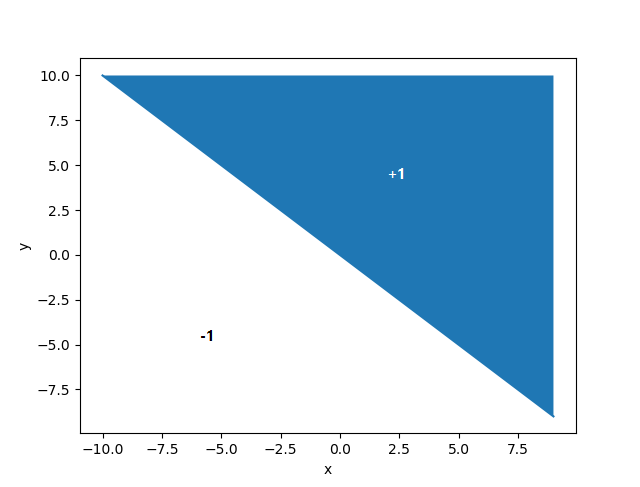
\includegraphics{p2_15.png}}
	\end{figure}
	\item Due to the hint, we can construct the first point randomly, and the generate the second point with larger x-component and smaller y-component. The third point we can generate will have a even larger x-component and even smaller y-component than the previous point. In this way we can generate infinite number of points, which means that $H$ can always shatter infinite number of points. SO, $d_{vc}=\infty$ and $m_H(N)=2^N$.
\end{enumerate}

\newpage

\noindent{\bf Problem 2.24}
\begin{enumerate} [(a)]
	\item For any two randomly chosen $D={(x_1,x_1^2),(x_2,x_2^2)}$, $g(x)$ should be the line connect this two points.\\
	\\Therefore,\[
		\begin{aligned}
			g(x)&=kx+b\\
			x^1_2&=kx_1+b\\
			x^2_2&=kx_2+b\\
		\end{aligned}
	\]
	So,\[
		g(x)=(x_1+x_2)x-x_1x_2
	\]

	According to the formula $\bar{g}(x)=\frac{1}{K}\sum^K_{k=1}g_k(x)$,
	\[
		\bar{g}(x)=\frac{1}{K}\sum^K_{k=1}[(x_{k1}+x_{k2})x-x_{k1}x_{k2}]=0
	\]
	\item \begin{enumerate}[(1)]
		\item To compute $\bar{g}(x)$, randomly select 2 points on [-1,1] and calculate $g(x)$ for this pair of points. Do the above step 10000 times and then calculate $\bar{g}(x)$ by using formula $\bar{g}(x)=\frac{1}{K}\sum^K_{k=1}g_k(x)$.
		\item To compute $E_{out}(g^D)$, there is a formula $E_{out}(g^D)=E_x[(g^D(x)-f(x))^2]$. So we can get $E_{out}$ by use this formula.
		\item for $bias$, use the formula $bias=(\bar{g}(x)-f(x))^2$ and $bias=E_x[bias(x)]$
		\item for $var$, use the formula $var(x)=E_x[var(x)]$ and $var=E_x[var(x)]$
	\end{enumerate}
	
	

	\item 
	\begin{figure}[htb]
		{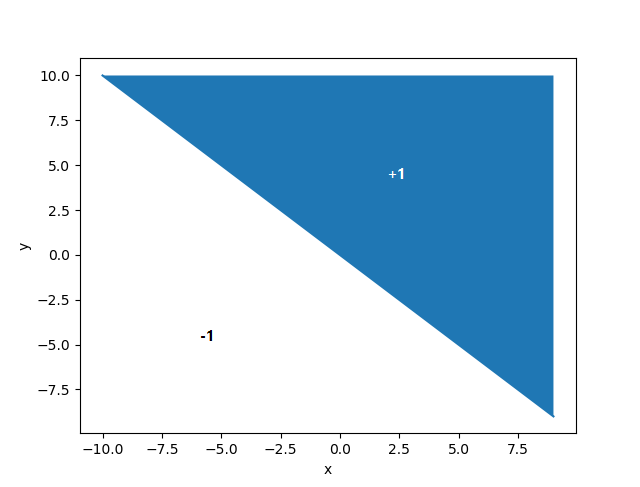
\includegraphics[height=10cm]{p2_15.png}}
	\end{figure}
	From the experiment:
	Eout is 0.5333333333333333\\
	bias is 0.19569357380857\\
	var is 0.33338149781948495\\
	So, $E[E_{out}]=bias+var$
	
	\newpage
	
	\item According to the formula mentioned in part(b),\[\
		\begin{aligned}
		E_{out}&=E_x[((x_1+x_2)x-x_1x_2-x^2)^2]\\
		&=\frac{1}{8}\int^1_{-1}\int^1_{-1}\int^1_{-1}[((x_1+x_2)x-x_1x_2-x^2)^2]dx_1dx_2dx\\
		&=0.533
		\end{aligned}
	\]
	\[
		\begin{aligned}
		bias&=E_x[(\bar{g}(x)-f(x))^2]\\
		&=\frac{1}{2}\int^1_{-1}(0-x^2)^2dx\\
		&=0.2
		\end{aligned}
	\]
	From part(a), we get $\bar{g}(x)=0$, so
	\[
		\begin{aligned}
		var(x)&=E_x[E_D[(g^D(x)-\bar{g}(x))^2]]\\
		&=\frac{1}{8}\int^1_{-1}\int^1_{-1}\int^1_{-1}[(x_1+x_2)x-x_1x_2]^2dx_1dx_2dx\\
		&=\frac{2}{3}x^2+\frac{1}{9}
		\end{aligned}
	\]
	\[
		\begin{aligned}
		var&=E_x[\frac{2}{3}x^2+\frac{1}{9}]\\
		&=\frac{1}{2}\int^1_{-1}\frac{2}{3}x^2+\frac{1}{9}\\
		&=\frac{1}{3}
		\end{aligned}
	\]
	Therefrore,\[
		E_{out} = 0.533=0.2+\frac{1}{3}=bias+var
	\]
\end{enumerate}
\newpage
\end{document}
\end{document}
